\subsubsection{DataAccess}
DataAccess implementerer IDataAccess og står for at skrive og læse data records til/fra databasen.
IDataAccess refereres af klassen SmartPoolDB. Klassen DataAccess kan ses på figur \ref{fig:dataAccessClassNoInherit}

\begin{figure}
\centering
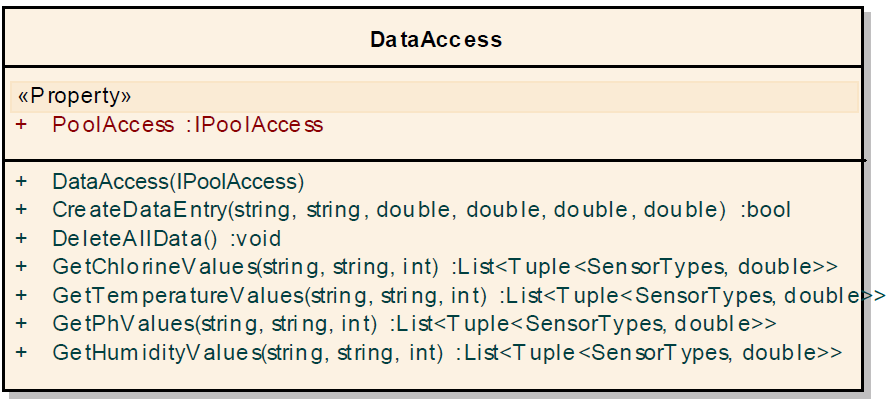
\includegraphics[width=0.7\linewidth]{figs/implementering/dataAccessClassNoInherit}
\caption{Klassen DataAccess}
\label{fig:dataAccessClassNoInherit}
\end{figure}


\paragraph{Metodebeskrivelser}

\subparagraph{CreateDataEntry}\

\textit{bool CreateDataEntry(string ownerEmail, string poolName, double chlorine, double temp, double pH, double humidity)}
\todo{do dis}


\subparagraph{DeleteAllData}\

\textit{void DeleteAllData()}
\todo{do dis}

\subparagraph{GetChlorineValues}\

\textit{List<Tuple<SensorTypes, double>> GetChlorineValues(string poolOwnerEmail, string poolName, int daysToGoBack)}
\todo{do dis}

\subparagraph{GetTemperatureValues}\

\textit{List<Tuple<SensorTypes, double>> GetTemperatureValues(string poolOwnerEmail, string poolName, int daysToGoBack)}
\todo{do dis}

\subparagraph{GetPhValues}\

\textit{List<Tuple<SensorTypes, double>> GetPhValues(string poolOwnerEmail, string poolName, int daysToGoBack)}
\todo{do dis}

\subparagraph{GetHumidityValues}\

\textit{List<Tuple<SensorTypes, double>> GetHumidityValues(string poolOwnerEmail, string poolName, int daysToGoBack);}
\todo{do dis}

\paragraph{Properties}

\subparagraph{PoolAccess}\

\textit{IPoolAccess PoolAccess { get; set; }}